\chapter{Requirements of MOM}
\label{chap:RequirMOM}

In the analysis we came to the conclusion that the following items is necessary for MOM: 
\begin{itemize}
	\item A device to toggle the power of an electronic media
	\item An individual key for each child that can be read by the device
	\item A website to set up rules, permissions and view/modify allowed usage of electronic media
\end{itemize} 


The first item is called controller in this system, the second is the tag and the last is the website on the computer. But also new components of the system is necessary. As explained in the previous section a daemon is needed to check the relevant rules and perform the appropriate actions if the conditions holds. Also during the following sections we find that a web service is needed. 

In the following sections the specification of the website, controller and tag, web service and daemon will be explained, before the design and implementation will be presented for each of them in the following chapters.  

\section{MOM's Website}
\label{section:momswebsite}
A Media-Online Management (MOM) owner needs a way to manage the system and for this a website will be made. There are several requirements for this website:

\begin{itemize}
	\item Register a new MOM together with a user profile which is a manager of this system
	\item Make it possible to add, edit and delete user profiles in an existing MOM 
	\item Make it possible to add, edit and delete Controllers from an existing MOM
	\item There should be a way to add, edit and delete Tags to the system. Also a tag should be connected to a user profile
	\item There need to be an option to add, edit and delete rules, permissions and chores from a system
	\item The user should be able to connect rules and permission with one or more user profiles. The connection should also be able to be removed without removing the rule or permission
	\item When a chore is done in the real world by a child profile then by connecting this profile to a chore, points should be added to his profile
\end{itemize}

There are also some requirements that is nice for the parents to use, but they are not essential for MOM system:

\begin{itemize}
	\item present the media consumption data as graphs or logs such that the parents easy can get an overview of their children's media consumption 
	\item present data from MOM in a calendar that shows rule and permission with profiles for whom this is relevant. The calendar should also show when a chore have been done and by who.
\end{itemize}

In chapter \vref{chap:website} the design and implementation of the website will be presented in more detail. 
 

\section{Tag and Controller}
The tag used in this system is using Radio-frequency Identification (RFID). The tag need to be uniquely identified in MOM and it must uniquely identify its user. The tag is used in combination with the controller.

The controller is an Arduino which is connected to a tag reader. Like the tag it need to be uniquely identified in MOM. The controller must be able to do the following.

\begin{itemize}
	\item Read the data from the tag
	\item Send and receive messages from the server
	\item Control the power source of the media 
	\item Temporarily store the tag id that activated this controller
	\item Keep track of the time spent between activation of the media to its end
\end{itemize}
 
The design and implementation of the controller will be explained further in chapter \vref{chap:controller}. 

The controller must communicate with the server and this is done via a web service.

\section{API}

The API is used to parse the relevant data to the controller. Its requirements are:

\begin{itemize}
	\item Receive and send messages to the controller
	\item From a tag and controller it should be able to determine whether a user may use the media which is connected to the controller
	\item It must be able to subtract points from a user after he has been using a media
	\item It should able to calculate when a controller should be turned off because of a rule, permission or point.
\end{itemize}

The web service's design and implementation is explained further in chapter \vref{chap:api}.


\section{Daemon}
The daemon is used to update data in the database from a rule which the user have made at some point. The daemon does not have any direct contact to a client. The daemon should handle any rule that is time determined so the condition is either Timestamp or Timeperiod. Then the daemon should do the appropriate action which could be add points to user or block a user.

The design and implementation of the daemon is presented in detail in chapter \vref{chap:daemon}. 
 
\section{System Architecture}
\label{sec:sysArchitecture}
Now that all subsystem of the Media-Online Management have been presented the overall system architecture can be explained. MOM is using the client server architecture which is shown in the figure \ref{fig:serveroverview} \citep{OOAD}. This system has two types of clients the first is a controller and the second is a computer where the user manages the system via the web site. The controller is depended on the web service on the server and the computer is depended on the web site. On the server there is the web site, web service and daemon which all are depended on the functions component, MySQLHelper class and data component. In the function component there are several functions to work on the data in the database and this component is depended on MySQLHelper because it should establish the database connection and parse the quires on to the database. 

\begin{figure}
	\centering
		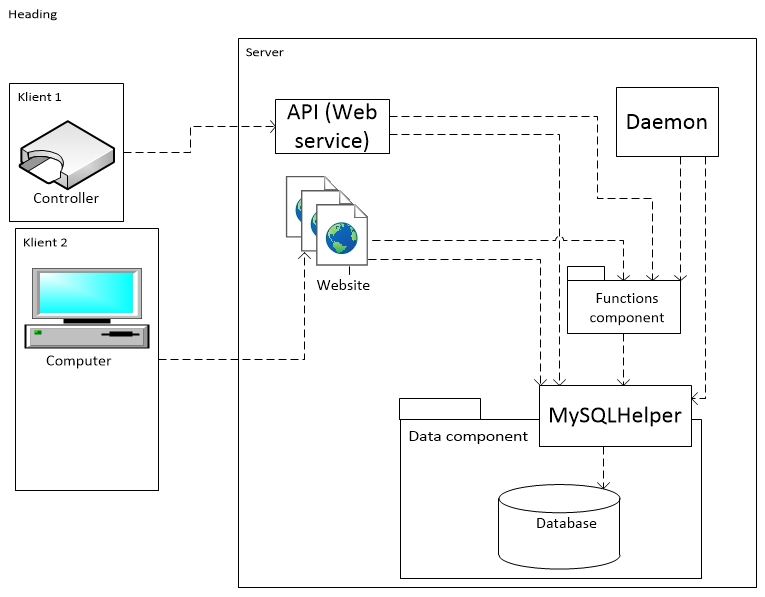
\includegraphics[width=1.25\textwidth,  angle=90]{images/serveroverview.jpg}
	\caption{system architecture}
	\label{fig:serveroverview}
\end{figure}

In the following chapters design and implementation of the web site, web service, deamon and database will be presented.

 


